% !TeX root = er.tex

\chapter{Navigation basée sur des cartes}\label{ch.map-based}
\index{navigation!basée sur la carte}

Maintenant que nous disposons d'une carte, qu'elle soit fournie par l'utilisateur ou découverte par le robot, nous pouvons discuter de \emph{la planification des itinéraires}, un algorithme de plus haut niveau. Prenons l'exemple d'un robot utilisé dans un hôpital pour transporter des médicaments et d'autres fournitures des zones de stockage vers les médecins et les infirmières. Étant donné l'une de ces tâches, quelle est la meilleure façon d'aller du point A au point B. Il peut y avoir plusieurs façons de se déplacer dans les couloirs pour atteindre l'objectif, mais il peut aussi y avoir des chemins courts que le robot n'est pas autorisé à emprunter, par exemple des chemins qui passent par les couloirs près des salles d'opération.

Nous présentons trois algorithmes de planification du chemin le plus court entre une position de départ \p{S} et une position d'arrivée \p{G}, en supposant que nous disposons d'une carte de la zone indiquant la position des obstacles qui s'y trouvent. Edsgar W. Dijkstra, l'un des pionniers de l'informatique, a proposé un algorithme pour le problème du plus court chemin. La section~\ref{s.dijkstra-grid} décrit l'algorithme pour une carte quadrillée, tandis que la section \ref{s.dijkstra-continuous} décrit l'algorithme pour une carte continue. L'algorithme~\ref{s.astar}, une amélioration de l'algorithme de Dijkstra basée sur des méthodes heuristiques, est présenté dans la section~ref{s.astar}. Enfin, la section~\ref{s.path-and-obstacle} explique comment combiner un algorithme de planification de chemin de haut niveau avec un algorithme d'évitement d'obstacles de bas niveau.

\section{Algorithme de Dijkstra pour une carte quadrillée} \label{s.dijkstra-grid}
\index{Algorithme de Dijkstra}

Dijkstra a décrit son algorithme pour un graphe discret de nœuds et d'arêtes. Nous le décrivons ici pour une grille de cellules (Fig.~\ref{fig.dijkstra-grid}). La cellule \p{S} est la cellule de départ du robot et sa tâche consiste à se déplacer jusqu'à la cellule d'arrivée \p{G}. Les cellules contenant des obstacles sont représentées en noir. Le robot peut détecter un \emph{voisin} de la cellule \p{c} qu'il occupe et s'y déplacer. Par souci de simplicité, nous précisons que les cellules voisines de \p{c} sont les quatre cellules qui lui sont adjacentes horizontalement et verticalement, mais pas en diagonale. La figure \ref{fig.dijkstra-path} montre le chemin le plus court entre \p{S} et \p{G} :
\[
\begin{array}{ll}
(4,0) \rightarrow &(4,1)\rightarrow (3,1) \rightarrow (2,1) \rightarrow (2,2) \rightarrow \\
&(2,3) \rightarrow (3,3) \rightarrow (3,4) \rightarrow (3,5) \rightarrow (4,5)\,.
\end{array}
\]
\begin{figure}
\begin{minipage}{.5\textwidth}
\begin{tikzpicture}[scale=.8]
\pic[scale=.8,draw] at (0,0) {astar};
\end{tikzpicture}
\caption{Carte de la grille de l'algorithme de Dijkstra}
%\caption{Grid map for Dijkstra's algorithm}
\label{fig.dijkstra-grid}
\end{minipage}
\hspace{\fill}
\begin{minipage}{.5\textwidth}
\begin{tikzpicture}[scale=.8]
\pic[scale=.8,draw] at (0,0) {astar};
\begin{scope}[xshift=.5cm,yshift=.5cm]
\draw[->,thick,blue] (.2,0) -- (1,0);
\draw[->,thick,blue] (1,0) -- (1,1);
\draw[->,thick,blue] (1,1) -- (1,2);
\draw[->,thick,blue] (1,2) -- (2,2);
\draw[->,thick,blue] (2,2) -- (3,2);
\draw[->,thick,blue] (3,2) -- (3,1);
\draw[->,thick,blue] (3,1) -- (4,1);
\draw[->,thick,blue] (4,1) -- (5,1);
\draw[->,thick,blue] (5,1) -- (5,.2);
\end{scope}
\end{tikzpicture}
\caption{Le plus court chemin trouvé par l'algorithme de Dijkstra}
%\caption{The shortest path found by Dijkstra's algorithm}
\label{fig.dijkstra-path}
\end{minipage}
\end{figure}

Deux versions de l'algorithme sont présentées : La première concerne les grilles où le coût de déplacement d'une cellule à l'une de ses voisines est constant. Dans la seconde version, chaque cellule peut avoir un coût différent associé à son déplacement, de sorte que le chemin le plus court géométriquement n'est pas nécessairement le plus court lorsque les coûts sont pris en compte.

\subsection{Algorithme de Dijkstra sur une carte quadrillée à coût constant}
\index{Algorithme de Dijkstra sur une carte quadrillée à coût constant}

L'algorithme~\ref{alg.dijkstra-grid} est l'algorithme de Dijkstra pour une carte quadrillée. L'algorithme est démontré sur la grille de $5\times 6$ cellules de la Fig.~\ref{fig.dijkstra-simple}. Trois obstacles sont représentés par les cellules noires.

\begin{figure}
\begin{alg}{Algorithme de Dijkstra sur une carte quadrillée}{dijkstra-grid}
&\idv{}integer n \ass 0&// Distance from start\\
&\idv{}cell array grid \ass all unmarked&// Grid map\\
&\idv{}cell list path \ass empty&// Shortest path\\
&\idv{}cell current&// Current cell in path\\
&\idv{}cell c&// Index over cells\\
&\idv{}cell S \ass $\cdots$&// Source cell\\
&\idv{}cell G \ass $\cdots$&// Goal cell\\
\hline
\stl{}&mark S with n&\\
\stl{}&while G is unmarked&\\
\stl{}&\idc{}n \ass n $+$ 1&\\
\stl{}&\idc{}for each unmarked cell c in grid&\\
\stl{}&\idc{}\idc{}\idc{}next to a marked cell&\\
\stl{}&\idc{}\idc{}mark c with n&\\
\stl{}&current \ass G&\\
\stl{}&append current to path&\\
\stl{}&while S not in path&\\
\stl{}&\idc{}append lowest marked neighbor c&\\
\stl{}&\idc{}\idc{}of current to path&\\
\stl{}&\idc{}current \ass c&\\
\end{alg}
\end{figure}

\begin{figure}
\begin{minipage}{.5\textwidth}
\begin{tikzpicture}[scale=.8]
\pic[scale=.8,draw] at (0,0) {astar};
\end{tikzpicture}
\caption{Carte quadrillée pour l'algorithme de Dijkstra}
%\caption{Grid map for Dijkstra's algorithm}
\label{fig.dijkstra-simple}
\end{minipage}
\hspace{\fill}
\begin{minipage}{.5\textwidth}
\begin{tikzpicture}[scale=.8]
\pic[scale=.8,draw] at (0,0) {astar};
\foreach \x/\y/\n in {0/0/0, 1/0/1, 0/1/1, 1/1/2, 0/2/2}
  \node at (\x+.2,\y+.8) {\p{\n}};
\end{tikzpicture}
\caption{Les deux premières itérations de l'algorithme de Dijkstra}
%\caption{The first two iterations of Dijkstra's algorithm}
\label{fig.dijkstra-simple-2}
\end{minipage}
\end{figure}

L'algorithme marque chaque cellule \p{c} du nombre d'étapes nécessaires pour atteindre \p{c} à partir de la cellule de départ \p{S}. Dans les figures, le nombre d'étapes est représenté par un chiffre dans le coin supérieur gauche d'une cellule. Dans un premier temps, la cellule \p{S} est marquée par $0$ car aucune étape n'est nécessaire pour atteindre \p{S} à partir de \p{S}. Ensuite, marquez chaque voisin de \p{S} avec $1$ puisqu'ils sont à un pas de \p{S} ; puis marquez chaque voisin d'une cellule marquée $1$ avec $2$. La figure \ref{fig.dijkstra-simple-2} montre la carte de la grille après ces deux itérations de l'algorithme.

\begin{figure}
\begin{minipage}{.5\textwidth}
\begin{tikzpicture}[scale=.8]
\pic[scale=.8,draw] at (0,0) {astar};
\foreach \x/\y/\n in {0/0/0, 1/0/1, 0/1/1, 1/1/2, 0/2/2, 0/3/3, 1/2/3, 0/4/4, 1/3/4, 2/2/4, 3/2/5, 1/4/5}
  \node at (\x+.2,\y+.8) {\p{\n}};
\end{tikzpicture}
\caption{Après cinq itérations de l'algorithme de Dijkstra}
%\caption{After five iterations of Dijkstra's algorithm}
\label{fig.dijkstra-simple-5}
\end{minipage}
\hspace{\fill}
\begin{minipage}{.5\textwidth}
\begin{tikzpicture}[scale=.8]
\foreach \x/\y in {0/0, 1/0, 1/1, 1/2, 2/2, 3/2, 3/1, 4/1, 5/1, 5/0}
  \draw[fill,lightgray] (\x,\y) rectangle +(1,1);
\pic[scale=.8,draw] at (0,0) {astar};
\foreach \x/\y/\n in {0/0/0, 1/0/1, 0/1/1, 1/1/2, 0/2/2, 0/3/3, 1/2/3, 0/4/4, 1/3/4, 2/2/4, 3/2/5, 1/4/5, 3/3/6, 3/1/6, 3/4/7, 3/0/7, 4/1/7, 4/3/7, 4/0/8, 5/3/8, 4/4/8, 5/1/8, 5/4/9, 5/0/9}
  \node at (\x+.2,\y+.8) {\p{\n}};
\end{tikzpicture}
\caption{La carte quadrillée finale avec le chemin le plus court marqué}
%\caption{The final grid map with the shortest path marked}
\label{fig.dijkstra-simple-9}
\end{minipage}
\end{figure}

L'algorithme se poursuit de manière itérative : si une cellule est marquée $n$, ses voisins non marqués sont marqués $n+1$. Lorsque \p{G} est finalement marquée, nous savons que la distance la plus courte entre \p{S} et \p{G} est de $n$. La figure \ref{fig.dijkstra-simple-5} montre la carte de la grille après cinq itérations et la figure \ref{fig.dijkstra-simple-9} montre la carte finale de la grille après neuf itérations, lorsque la cellule cible a été atteinte.

Il est maintenant facile de trouver le chemin le plus court en travaillant à rebours à partir de la cellule cible \p{G}. Dans la figure \ref{fig.dijkstra-simple-9}, le chemin le plus court est constitué des cellules colorées en gris. En partant de la cellule but à la coordonnée $(4,5)$, la cellule précédente doit être soit $(4,4)$, soit $(3,5)$, puisqu'elles sont à huit pas du point de départ. (Nous choisissons arbitrairement $(3,5)$. A partir de chaque cellule sélectionnée marquée $n$, nous choisissons une cellule marquée $n-1$ jusqu'à ce que la cellule \p{S} marquée $0$ soit sélectionnée. La liste des cellules sélectionnées est la suivante :
\[
(4,5),\, (3,5),\, (3,4),\, (3,3),\, (2,3),\, (2,2),\, (2,1),\, (3,1),\, (4,1),\, (4,0)\,.
\]
En inversant la liste, on obtient le plus court chemin de \p{S} à \p{G}. Vérifiez qu'il s'agit du même chemin que celui que nous avons trouvé intuitivement (Fig.~\ref{fig.dijkstra-path}).

\noindent\textbf{Exemple} La figure~\ref{fig.dijkstra} montre comment l'algorithme de Dijkstra fonctionne sur un exemple plus compliqué. La carte quadrillée comporte $16 fois 16$ cellules et la cellule cible \p{G} est entourée d'un obstacle et difficile à atteindre. Le diagramme supérieur gauche montre la carte de la grille après trois itérations et le diagramme supérieur droit montre la carte après $19$ itérations. L'algorithme procède maintenant à l'exploration des cellules autour des deux côtés de l'obstacle. Enfin, dans le diagramme inférieur gauche, \p{G} est trouvé après $25$ itérations, et le chemin le plus court est indiqué en gris dans le diagramme inférieur droit. Nous voyons que l'algorithme n'est pas très efficace pour cette carte : bien que le chemin le plus court ne représente que $25$ étapes, l'algorithme a exploré $256-25=231$ cellules !

\begin{figure}
\begin{center}
\includegraphics[width=.9\textwidth]{grid-plan.pdf}
\end{center}
\caption{Algorithme de Dijkstra pour la planification d'un chemin sur une carte quadrillée. Les quatre étapes de l'exécution de l'algorithme sont représentées à partir du diagramme supérieur gauche.}\label{fig.dijkstra}
\end{figure}

\subsection{Algorithme de Dijkstra avec coûts variables}
\index{Algorithme de Dijkstra!grille avec coûts variables}

L'algorithme~\ref{alg.dijkstra-grid} et l'exemple de la Fig.~\ref{fig.dijkstra} supposent que le coût d'un pas d'une cellule à l'autre est constant : la ligne trois de l'algorithme ajoute $1$ au coût pour chaque voisin. L'algorithme de Dijkstra peut être modifié pour prendre en compte un coût variable pour chaque étape. Supposons qu'une zone de l'environnement soit recouverte de sable et qu'il soit plus difficile pour le robot de se déplacer dans cette zone. Dans l'algorithme, au lieu d'ajouter $1$ au coût de chaque cellule voisine, nous pouvons ajouter $k$ à chaque cellule sablonneuse voisine pour refléter le coût supplémentaire.

\begin{figure}
\begin{center}
\includegraphics[width=.9\textwidth]{grid-plad-sand.pdf}
\end{center}
\caption{Algorithme de Dijkstra avec un coût variable par cellule (diagramme de gauche, coût=$4$, diagramme de droite, coût=$2$)}\label{fig.path-sand}
\end{figure}

La grille de gauche de la Fig.~\ref{fig.path-sand} comporte quelques cellules marquées d'une ligne diagonale pour indiquer qu'elles sont recouvertes de sable et que le coût du déplacement à travers elles est de $4$ et non de $1$. Le chemin le plus court, marqué en gris, comporte $17$ étapes et coûte également $17$ puisqu'il contourne le sable.

Le chemin le plus court dépend du coût attribué à chaque cellule. Le diagramme de droite montre le chemin le plus court si le coût du passage dans une cellule contenant du sable n'est que de $2$. Le chemin fait $12$ pas, mais son coût est de $14$ pour tenir compte du fait qu'il faut faire deux pas dans le sable.

\begin{framed}
\act{Algorithme de Dijkstra sur une carte quadrillée}{dijkstra-grid}
\begin{itemize}
\item Construire une carte quadrillée et appliquer l'algorithme de Dijkstra.
\item Modifier la carte pour inclure des cellules à coût variable et appliquer l'algorithme.
\item Mettre en œuvre l'algorithme de Dijkstra.
\begin{itemize}
\item Créer une grille sur le sol.
\item Ecrire un programme qui permet au robot de se déplacer d'une cellule de départ connue à une cellule d'arrivée connue. Puisque le robot doit mémoriser sa position actuelle, utilisez-la pour créer une carte des cellules qu'il a traversées.
\item Placez quelques obstacles dans la grille et inscrivez-les dans la carte du robot.
\end{itemize}
\end{itemize}
\end{framed}

\section{Algorithme de Dijkstra pour une carte continue}\label{s.dijkstra-continuous}
\index{Dijkstra's algorithm!continuous map}

Dans une carte continue, la zone est un plan géométrique ordinaire à deux dimensions. Une approche de l'utilisation de l'algorithme de Dijkstra dans une carte continue consiste à transformer la carte en un graphe discret en traçant des lignes verticales à partir des bords supérieur et inférieur de l'environnement jusqu'à chaque coin d'un obstacle. La zone est ainsi divisée en un nombre fini de segments, chacun d'entre eux pouvant être représenté comme un nœud dans un graphe. Le diagramme de gauche de la Fig.~\ref{fig.map-graph-at} montre sept lignes verticales qui divisent la carte en dix segments qui sont représentés dans le graphique de la Fig.~\ref{fig.map-graph-ab}. Les arêtes du graphique sont définies par la relation d'adjacence des segments. Il existe une arête dirigée du segment \p{A} vers le segment \p{B} si \p{A} et \p{B} partagent une frontière commune. Par exemple, il existe des arêtes entre le nœud $2$ et les nœuds $1$ et $3$ puisque les segments correspondants partagent une arête avec le segment $2$.

\begin{figure}
\begin{center}
\includegraphics[width=\textwidth]{plan-continuous2at.pdf}
\end{center}
\caption{Segmentation d'une carte continue par des lignes verticales et chemin à travers les segments}\label{fig.map-graph-at}
\end{figure}

\begin{figure}
\begin{center}
\includegraphics[width=.8\textwidth]{plan-continuous2ab.pdf}
\end{center}
\caption{Le graphique construit à partir de la carte continue segmentée}\label{fig.map-graph-ab}
\end{figure}

Quel est le chemin le plus court entre le sommet $2$ représentant le segment contenant le point de départ et le sommet $10$ représentant le segment contenant le but ? Le résultat de l'application de l'algorithme de Dijkstra est $\p{S} \rightarrow 2\rightarrow 3\rightarrow 6\rightarrow 9\rightarrow 10 \rightarrow \p{G}$. Bien qu'il s'agisse du chemin le plus court en termes de nombre d'arêtes du graphe, ce n'est pas le chemin le plus court dans l'environnement. La raison en est que nous avons attribué un coût constant à chaque arête, bien que les segments de la carte soient de tailles différentes. 

Étant donné que chaque sommet représente un grand segment de l'environnement, nous devons savoir comment le déplacement d'un sommet à un autre se traduit par le déplacement d'un segment à un autre. Le diagramme de droite de la figure \ref{fig.map-graph-at} montre une possibilité : chaque segment est associé à son centre géométrique, indiqué par l'intersection des lignes diagonales en pointillés dans la figure. Le chemin dans l'environnement associé au chemin dans le graphique va du centre d'un segment au centre du segment suivant, sauf que les positions de départ et d'arrivée sont à leurs emplacements géométriques. Bien que cette méthode soit raisonnable sans connaissance supplémentaire de l'environnement, elle ne donne pas le chemin optimal qui doit rester proche des limites des obstacles.

La figure~\ref{fig.map-graph-bt} montre une autre approche de la planification des chemins dans une carte continue. Elle utilise un \emph{graphique de visibilité}\index{cartographie!graphique de visibilité}, où chaque sommet du graphique représente un coin d'un obstacle, et il y a des sommets pour les positions de départ et d'arrivée. Il existe une arête entre le sommet $v_1$ et le sommet $v_2$ si les coins correspondants sont visibles. Par exemple, il y a une arête $C\rightarrow E$ parce que le coin $E$ de l'obstacle de droite est visible depuis le coin $C$ de l'obstacle de gauche. La figure~\ref{fig.map-graph-bb} montre le graphe formé par ces nœuds et ces arêtes. Il représente tous les candidats au chemin le plus court entre le point de départ et le point d'arrivée.

\begin{figure}
\begin{center}
\includegraphics[width=\textwidth]{plan-continuous2bt.pdf}
\end{center}
\caption{Une carte continue avec des lignes d'un coin à l'autre et le chemin à travers les coins.}\label{fig.map-graph-bt}
\end{figure}

\begin{figure}
\begin{center}
\includegraphics[width=.7\textwidth]{plan-continuous2bb.pdf}
\end{center}
\caption{Le graphique construit à partir de la carte continue segmentée}
\label{fig.map-graph-bb}
\end{figure}

Il est facile de voir que les chemins dans le graphique représentent des chemins dans l'environnement, puisque le robot peut simplement se déplacer d'un coin à l'autre. Ces chemins sont les plus courts car aucun chemin, disons de $A$ à $B$, ne peut être plus court que la ligne droite de $A$ à $B$. L'algorithme de Dijkstra donne le chemin le plus court sous la forme $S\rightarrow D\rightarrow F\rightarrow H\rightarrow G$. Dans ce cas, le chemin le plus court en termes de nombre d'arêtes est également le chemin le plus court géométriquement.

Bien qu'il s'agisse du chemin le plus court, un robot réel ne peut pas suivre ce chemin parce qu'il a une taille finie et que son centre ne peut pas suivre le bord d'un obstacle. Le robot doit maintenir une distance minimale par rapport à chaque obstacle, ce qui peut être réalisé en augmentant la taille des obstacles de la taille du robot (diagramme de droite de la Fig.~\ref{fig.map-graph-bb}). Le chemin obtenu est optimal et peut être parcouru par le robot.

\begin{framed}
\act{Algorithme de Dijkstra pour les cartes continues}{dijkstra-continuous}
\begin{itemize}
\item Dessinez une version plus grande de la carte de la Fig.~\ref{fig.map-graph-bt}. Mesurez la longueur de chaque segment. Appliquez maintenant l'algorithme de Dijkstra pour déterminer le chemin le plus court.
\item Créez votre propre carte continue, extrayez le graphe de visibilité et appliquez l'algorithme de Dijkstra.
\end{itemize}
\end{framed}

\section{Planification de trajectoire avec l'algorithme \astar{}}\label{s.astar}
\index{A* algorithm}

L'algorithme de Dijkstra recherche la cellule cible dans toutes les directions ; cela peut être efficace dans un environnement complexe, mais ce n'est pas le cas lorsque le chemin est simple, par exemple une ligne droite jusqu'à la cellule cible. Regardez le diagramme en haut à droite de la figure \ref{fig.dijkstra} : près du coin supérieur droit de l'obstacle central, il y a une cellule à une distance de $19$ de la cellule de départ. Après deux pas supplémentaires vers la gauche, il y aura une cellule marquée $21$ qui a un chemin vers la cellule de but qui n'est pas bloqué par un obstacle. Il n'y a manifestement aucune raison de continuer à explorer la région située à gauche de la grille, mais l'algorithme de Dijkstra continue à le faire. Il serait plus efficace si l'algorithme savait d'une manière ou d'une autre qu'il est proche de la cellule cible.

L'algorithme \emph{\astar{}} (prononcé "étoile") est similaire à l'algorithme de Dijkstra, mais il est souvent plus efficace car il utilise des informations supplémentaires pour guider la recherche. L'algorithme \astar{} prend en compte non seulement le nombre de pas à partir de la cellule de départ, mais aussi une \emph{fonction heuristique} qui donne une indication de la direction préférée de la recherche. Auparavant, nous utilisions une fonction de coût $g(x,y)$ qui donne le nombre réel de pas à partir de la cellule de départ. L'algorithme de Dijkstra étend la recherche en commençant par les cellules marquées par les valeurs les plus élevées de $g(x,y)$. Dans l'algorithme \astar{}, la fonction de coût $f(x,y)$ est calculée en ajoutant les valeurs d'une fonction heuristique $h(x,y)$ :
\[
f(x,y) = g(x,y) + h(x,y)\,.
\]

Nous démontrons l'algorithme \astar{} en utilisant comme fonction heuristique le nombre d'étapes entre la cellule cible \p{G} et la cellule $(x,y)$ \emph{sans tenir compte des obstacles}. Cette fonction peut être précalculée et reste disponible tout au long de l'exécution de l'algorithme. Pour la carte quadrillée de la Fig.~\ref{fig.dijkstra-simple}, la fonction heuristique est présentée dans la Fig.~\ref{fig.heuristic}.

\begin{figure}
\begin{minipage}{.48\textwidth}
\begin{tikzpicture}[scale=.65]
\pic[scale=.8,draw] at (0,0) {astar};
\foreach \x/\y/\n in {0/0/5, 1/0/4, 0/1/6, 1/1/5, 0/2/7, 0/3/8, 1/2/6, 0/4/9, 1/3/7, 2/2/5, 3/2/4, 1/4/8, 3/3/5, 3/1/3, 3/4/6, 3/0/2, 4/1/2, 4/3/4, 4/0/1, 5/3/3, 4/4/5, 5/1/1, 5/4/4, 5/0/0}
  \node at (\x+.8,\y+.2) {\p{\n}};
\end{tikzpicture}
\caption{Fonction heuristique}
%\caption{Heuristic function}
\label{fig.heuristic}
\end{minipage}
\hspace{\fill}
\begin{minipage}{.48\textwidth}
\begin{tikzpicture}[scale=.65]
\pic[scale=.8,draw] at (0,0) {astar};
\foreach \x/\y/\n in {0/0/5, 1/0/4, 0/1/6, 1/1/5, 0/2/7, 0/3/8, 1/2/6, 0/4/9, 1/3/7, 2/2/5, 3/2/4, 1/4/8, 3/3/5, 3/1/3, 3/4/6, 3/0/2, 4/1/2, 4/3/4, 4/0/1, 5/3/3, 4/4/5, 5/1/1, 5/4/4, 5/0/0}
  \node at (\x+.8,\y+.2) {\p{\n}};
\foreach \x/\y/\n in {0/0/0, 1/0/1, 0/1/1, 1/1/2}
  \node at (\x+.2,\y+.8) {\p{\n}};
\foreach \x/\y/\n in {0/0/5, 1/0/5, 0/1/7, 1/1/7}
  \node at (\x+.8,\y+.8) {\p{\n}};
\end{tikzpicture}
\caption{Les deux premières itérations de l'algorithme \astar{}}
%\caption{The first two iterations of the \astar{} algorithm}
\label{fig.astar2}
\end{minipage}
\end{figure}

Dans les diagrammes, nous garderons trace des valeurs des trois fonctions $f,g,h$ en les affichant dans différents coins de chaque cellule :
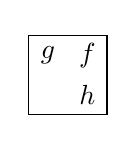
\begin{tikzpicture}[baseline=4mm]
\path (0,11mm) -- (1,1mm);
\draw (0,0) rectangle +(1,1);
\node at (.75,.25) {$h$};
\node at (.25,.75) {$g$};
\node at (.75,.75) {$f$};
\path (0,-1mm) -- (1,-1mm);
\end{tikzpicture}

La figure \ref{fig.astar2} montre la carte de la grille après deux étapes de l'algorithme \astar{}. Les cellules $(3,1)$ et $(3,0)$ reçoivent le même coût $f$ : l'une est plus proche de \p{S} (par le nombre d'étapes comptées) et l'autre est plus proche de \p{G} (par l'heuristique), mais toutes deux ont le même coût de $7$.

L'algorithme doit maintenir une structure de données des \emph{cellules ouvertes}, les cellules qui n'ont pas encore été développées. Nous utilisons la notation $(r,c,v)$, où $r$ et $c$ sont la ligne et la colonne de la cellule et $v$ est la valeur $f$ de la cellule. Chaque fois qu'une cellule ouverte est développée, elle est supprimée de la liste et les nouvelles cellules sont ajoutées. La liste est ordonnée de manière à ce que les cellules ayant les valeurs les plus faibles apparaissent en premier, ce qui facilite le choix de la cellule à développer ensuite. Les trois premières listes correspondant à la Fig.~\ref{fig.astar2} sont :
\begin{displaymath}
\begin{array}{l}
(4,0,5)\\
(4,1,5),\,(3,0,7)\\
(3,0,7),\,(3,1,7)\,.
\end{array}
\end{displaymath}

\begin{figure}
\begin{minipage}{.48\textwidth}
\begin{tikzpicture}[scale=.8]
\pic[scale=.8,draw] at (0,0) {astar};
\foreach \x/\y/\n in {0/0/5, 1/0/4, 0/1/6, 1/1/5, 0/2/7, 0/3/8, 1/2/6, 0/4/9, 1/3/7, 2/2/5, 3/2/4, 1/4/8, 3/3/5, 3/1/3, 3/4/6, 3/0/2, 4/1/2, 4/3/4, 4/0/1, 5/3/3, 4/4/5, 5/1/1, 5/4/4, 5/0/0}
  \node at (\x+.8,\y+.2) {\p{\n}};
\foreach \x/\y/\n in {0/0/0, 1/0/1, 0/1/1, 1/1/2, 0/2/2, 1/2/3, 2/2/4, 0/3/3, 1/3/4, 3/2/5, 3/3/6, 3/1/6}
  \node at (\x+.2,\y+.8) {\p{\n}};
\foreach \x/\y/\n in {0/0/5, 1/0/5, 0/1/7, 1/1/7, 0/2/9, 1/2/9, 2/2/9, 0/3/11, 1/3/11, 3/2/9, 3/3/11, 3/1/9}
  \node at (\x+.8,\y+.8) {\p{\n}};
\end{tikzpicture}
\caption{L'algorithme \astar{} après $6$ étapes}
%\caption{The \astar{} algorithm after $6$ steps}
\label{fig.astar6}
\end{minipage}
\hspace{\fill}
\begin{minipage}{.48\textwidth}
\begin{tikzpicture}[scale=.8]
\foreach \x/\y in {0/0, 1/0, 1/1, 1/2, 2/2, 3/2, 3/1, 4/1, 5/1, 5/0}
  \draw[fill,lightgray] (\x,\y) rectangle +(1,1);
\pic[scale=.8,draw] at (0,0) {astar};
\foreach \x/\y/\n in {0/0/5, 1/0/4, 0/1/6, 1/1/5, 0/2/7, 0/3/8, 1/2/6, 0/4/9, 1/3/7, 2/2/5, 3/2/4, 1/4/8, 3/3/5, 3/1/3, 3/4/6, 3/0/2, 4/1/2, 4/3/4, 4/0/1, 5/3/3, 4/4/5, 5/1/1, 5/4/4, 5/0/0}
  \node at (\x+.8,\y+.2) {\p{\n}};
\foreach \x/\y/\n in {0/0/0, 1/0/1, 0/1/1, 1/1/2, 0/2/2, 1/2/3, 2/2/4, 0/3/3, 1/3/4, 3/2/5, 3/3/6, 3/1/6, 3/0/7, 4/1/7, 4/0/8, 5/1/8, 5/0/9}
  \node at (\x+.2,\y+.8) {\p{\n}};
\foreach \x/\y/\n in {0/0/5, 1/0/5, 0/1/7, 1/1/7, 0/2/9, 1/2/9, 2/2/9, 0/3/11, 1/3/11, 3/2/9, 3/3/11, 3/1/9, 3/0/9, 4/1/9, 4/0/9, 5/1/9, 5/0/9}
  \node at (\x+.8,\y+.8) {\p{\n}};
\end{tikzpicture}
\caption{L'algorithme \astar{} atteint la cellule cible et trouve le chemin le plus court}
%\caption{The \astar{} algorithm reaches the goal cell and finds a shortest path}
\label{fig.astar9}
\end{minipage}
\end{figure}

La figure~\ref{fig.astar6} montre la carte de la grille après six étapes. On peut s'en rendre compte en regardant les valeurs $g$ dans le coin supérieur gauche de chaque cellule. La liste actuelle des cellules ouvertes est la suivante :
\[
(3,3,9),\, (1,0,11),\, (1,1,11),\, (1,3,11)\,.
\]
L'algorithme \astar{} choisit d'étendre la cellule $(3,3,9)$ avec le $f$ le plus bas. Les autres cellules de la liste ont une valeur $f$ de $11$ et sont ignorées, du moins pour l'instant. En continuant (Fig.~\ref{fig.astar9}), la cellule but est atteinte avec une valeur $f$ de $9$ et un plus court chemin en gris est affiché. La dernière liste avant d'atteindre le but est la suivante :
\[
(3,5,9),\, (4,4,9),\, (1,0,11),\, (1,1,11),\, (1,3,11)\,.
\]
Peu importe lequel des nœuds de valeur $9$ est choisi : dans les deux cas, l'algorithme atteint la cellule but $(4,5,9)$.

Toutes les cellules en haut à droite de la grille ne sont pas explorées car la cellule $(1,3)$ a une valeur $f$ de $11$ et ce ne sera jamais la plus petite valeur. Alors que l'algorithme de Dijkstra a exploré l'ensemble des $24$ cellules non-obstacles, l'algorithme \astar{} n'a exploré que $17$ cellules.

\subsubsection*{Un exemple plus complexe de l'algorithme \astar{}}

Appliquons l'algorithme \astar{} à la grille de la Fig.~\ref{fig.path-sand}. Rappelons que cette grille comporte du sable sur certaines de ses cellules, de sorte que la fonction $g$ donnera des valeurs plus élevées pour le coût de déplacement vers ces cellules. Le diagramme supérieur gauche de la figure \ref{fig.a-star} montre la fonction $g$ telle qu'elle est calculée par l'algorithme de Dijkstra, tandis que le diagramme supérieur droit montre la fonction heuristique $h$, le nombre de pas à partir du but en l'absence d'obstacles et de sable. Le reste de la figure montre quatre étapes de l'algorithme conduisant au chemin le plus court vers le but.

\begin{figure}
\begin{center}
\includegraphics[width=0.8\textwidth]{a-star-sand.pdf}
\end{center}
\caption{L'algorithme \astar{}. En haut à gauche : le nombre d'étapes jusqu'à l'objectif. En haut à droite : la fonction heuristique. Les diagrammes du milieu et du bas montrent quatre étapes de l'algorithme.}\label{fig.a-star}
\end{figure}

Dès le diagramme du milieu à gauche, nous voyons qu'il n'est pas nécessaire de chercher en haut à gauche, car les valeurs $f$ des cellules au-dessus et à gauche de \p{S} sont plus élevées que les valeurs à droite et en dessous de \p{S}. Dans le diagramme du milieu à droite, la première cellule de sable a une valeur de $13$, de sorte que l'algorithme continue d'étendre les cellules ayant un coût inférieur de $12$ vers la gauche. Dans le diagramme en bas à gauche, nous voyons que la recherche ne se poursuit pas jusqu'en bas à gauche de la carte parce que le coût de $16$ est plus élevé que le coût de $14$ une fois que la recherche quitte le sable. À partir de là, la cellule cible \p{G} est trouvée très rapidement. Comme dans l'algorithme de Dijkstra, le chemin le plus court est trouvé en repassant par les cellules ayant les valeurs $g$ les plus faibles jusqu'à ce que la cellule de départ soit atteinte.

En comparant les figures \ref{fig.dijkstra} et \ref{fig.a-star}, nous constatons que l'algorithme \astar{} n'a eu besoin de visiter que 71\% des cellules visitées par l'algorithme de Dijkstra. Bien que l'algorithme \astar{} doive effectuer un travail supplémentaire pour calculer la fonction heuristique, le nombre réduit de cellules visitées rend l'algorithme plus efficace. En outre, cette fonction heuristique ne dépend que de la zone explorée et non des obstacles ; même si l'ensemble des obstacles est modifié, il n'est pas nécessaire de recalculer la fonction heuristique.

\begin{framed}
\act{A* algorithme}{astar}
\begin{itemize}
\item Appliquer l'algorithme \astar{} et l'algorithme de Dijkstra sur une petite carte sans obstacles : placer la cellule de départ au centre de la carte et le but dans une cellule arbitraire. Comparez les résultats des deux algorithmes. Expliquez vos résultats. Le résultat dépend-il de la position de la cellule du but ?
\item Définir d'autres fonctions heuristiques et comparer les résultats des algorithmes \astar{} sur les exemples de ce chapitre.
\end{itemize}
\end{framed}

\section{Path following and obstacle avoidance}\label{s.path-and-obstacle}
\index{path following and obstacle avoidance}

Ce chapitre et les précédents ont abordé deux tâches différentes mais liées : la planification de la trajectoire à haut niveau et l'évitement des obstacles à bas niveau. Comment intégrer ces deux tâches ? L'approche la plus simple consiste à donner la priorité à l'algorithme de bas niveau (Fig.~\ref{fig.integrate-pp}). De toute évidence, il est plus important d'éviter de heurter un piéton ou de contourner un nid-de-poule que d'emprunter le chemin le plus court pour se rendre à l'aéroport. Le robot est normalement dans l'état \p{drive}, mais si un obstacle est détecté, il passe à l'état \p{avoid obstacle}. Ce n'est que lorsque l'obstacle a été franchi qu'il revient à l'état \p{planifier le chemin} afin que le chemin puisse être recalculé.

\begin{figure}
\begin{center}
\begin{tikzpicture}[scale=.8,node distance = 2cm and 4cm,align=left,minimum size=16mm]
\node[draw,circle] (plan)  {\p{plan}\\\p{chemin}};
\node[draw,circle] (drive) [right=of plan] {\p{conduire}};
\draw[->] (plan) to node[above,yshift=-4mm] {\p{vrai}$\leadsto$ \\ \p{passer à l'objectif}} (drive);
\draw[<-] (plan) to (180:15mm);
\node[draw,circle] (avoid) [below=of drive] {\p{éviter}\\\p{l'obstacle}};
\draw[->] (drive) to node[left,yshift=2mm] {\p{l'obstacle détecté} $\leadsto$ \\ \p{contourner l'obstacle}} (avoid);
\draw[->,bend left=20] (avoid) to node[left,xshift=-6mm] {\p{obstacle franchi} $\leadsto$\\\p{[pas d'action]}} (plan);
\end{tikzpicture}
\caption{Intégration de la planification de la trajectoire et de l'évitement des obstacles}
\label{fig.integrate-pp}
\end{center}
\end{figure}

La stratégie d'intégration des deux algorithmes dépend de l'environnement. La réparation d'une route peut prendre plusieurs semaines, il est donc logique d'ajouter l'obstacle à la carte. L'algorithme de planification de trajectoire tiendra compte de l'obstacle et la trajectoire résultante sera probablement meilleure qu'une trajectoire modifiée à la dernière minute par un algorithme d'évitement d'obstacles. À l'autre extrême, s'il y a beaucoup d'obstacles mobiles tels que des piétons traversant une rue, l'algorithme d'évitement d'obstacles pourrait simplement arrêter de se déplacer et attendre que les obstacles s'éloignent. Le plan initial peut alors être repris sans détour.

\begin{framed}
\act{Combinaison de la planification de la trajectoire et de l'évitement des obstacles}{combi}
\begin{itemize}
\item Modifiez votre implémentation de l'algorithme de suivi de ligne afin que le robot se comporte correctement même si un obstacle est placé sur la ligne. Essayez plusieurs des approches énumérées dans cette section.
\item Modifiez votre implémentation de l'algorithme de suivi de ligne afin que le robot se comporte correctement même si d'autres robots se déplacent de manière aléatoire dans la zone de la ligne. Veillez à ce que les robots ne se heurtent pas les uns aux autres.
\end{itemize}
\end{framed}

\section{Résumé}

La planification de trajectoire est un comportement de haut niveau d'un robot mobile : trouver le chemin le plus court d'un point de départ à un point d'arrivée dans l'environnement. La planification du chemin est basée sur une carte montrant les obstacles. L'algorithme de Dijkstra étend le chemin le plus court à toutes les cellules rencontrées jusqu'à présent. L'algorithme \astar{} réduit le nombre de cellules visitées en utilisant une fonction heuristique qui indique la direction vers la cellule cible.

La planification des chemins est basée sur un graphe tel qu'une carte quadrillée, mais elle peut également être réalisée sur une carte continue en créant un graphe d'obstacles à partir de la carte. Les algorithmes peuvent prendre en compte des coûts variables pour visiter chaque cellule.

L'évitement des obstacles à bas niveau doit être intégré dans la planification des chemins à haut niveau.

\section{Lecture complémentaire}

L'algorithme de Dijkstra est présenté dans tous les manuels sur les structures de données et les algorithmes, par exemple, \cite[Sect.~24.3]{crls3}. Les algorithmes de recherche tels que l'algorithme \astar{} sont un sujet central de l'intelligence artificielle \cite[Sect.~3.5]{ai}.
